




O \textit{C99}, assim como outros métodos baseados em divisão, tem sua performance fortemente influenciado pela quantidade segmentos desejados. Esses métodos alcançam melhores resultados em contextos onde a quantidade de segmentos é conhecida~\cite{Bokaei2015,Ferret2009,Kern2009,Naili2016}. Na Figura~\ref{fig:influencia-NSegs-WD} é mostrado a variação de \textit{WindowDiff} em função da quantidade de segmentos solicitada ao algoritmo. Observa-se que há um ponto ótimo próximo 0,45 indicando que para o conjunto de atas analisado o método dá melhores resultados com número de segmentos desejados próximo a 45\% do número de sentenças.

  \begin{figure}[!h]
	  \centering
	  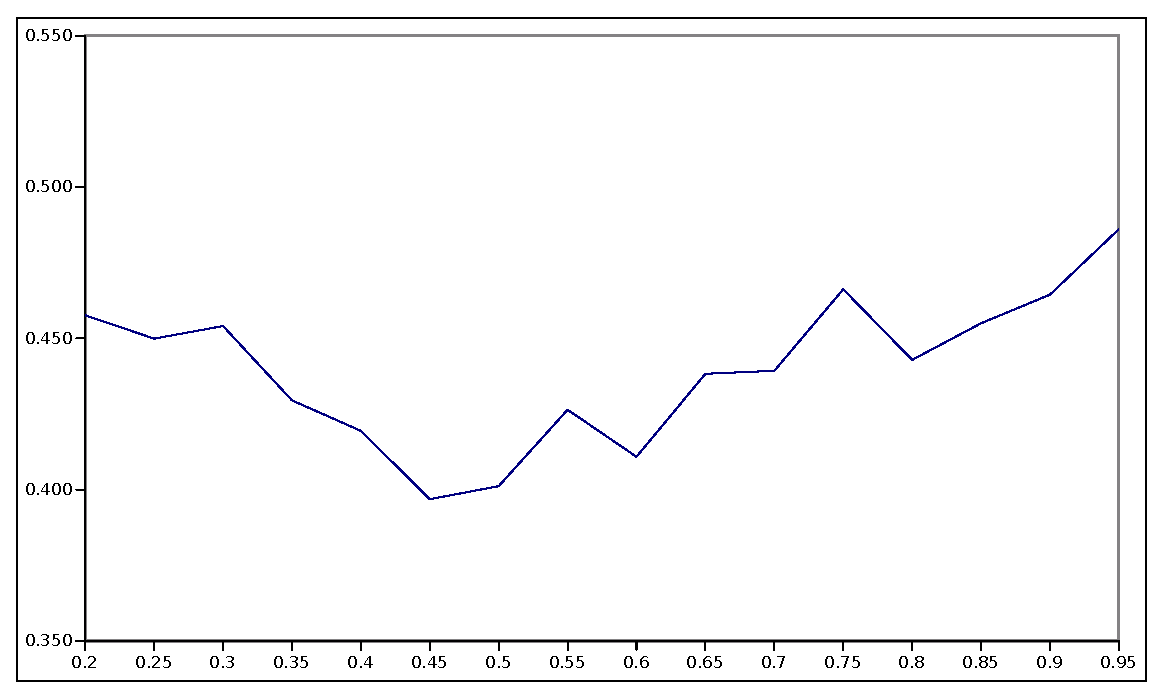
\includegraphics[width=0.9\textwidth]{conteudo/capitulos/figs/influencia-qtd-Segs-WD-C99.eps}
	  \caption{Influência da quantidade de segmentos em \textit{WindowDiff}}
	  \label{fig:influencia-NSegs-WD}
  \end{figure}






















